 \documentclass[10pt]{article}
\usepackage[utf8]{inputenc}
\usepackage{natbib}
\usepackage{graphicx}
\usepackage[margin=0.75in]{geometry}
\usepackage{url}
\usepackage{amsmath}
\usepackage{comment}
\usepackage[utf8]{inputenc}
\usepackage[T1]{fontenc}
%\usepackage[font={small,it}]{caption}
%\usepackage[font={it}]{caption}
%\usepackage{fancyhdr}
%\pagestyle{fancy}
%\fancyhf{}
%\lfoot{Iain Mclaughlan}
%\rfoot{s1524154}

\usepackage{listings}
\usepackage{color}
 
\definecolor{codegreen}{rgb}{0,0.6,0}
\definecolor{codegray}{rgb}{0.5,0.5,0.5}
\definecolor{codepurple}{rgb}{0.58,0,0.82}
\definecolor{backcolour}{rgb}{0.95,0.95,0.92}

\title{Precision Refrigerator}
\author{Iain McLaughlan\\ s1524154 }
\date{\today}

\begin{document}

\maketitle
\begin{abstract}
A precision refrigerator was built and controlled using a raspberry pi to precisely control the temperature of wine (water) by toggling the on/off state of a Peltier cooling unit. The efficiency of this cooling unit was then tested by comparing the energy consumed to change the temperature of the water with the specific heat capacity of water. The fridge was found to have a percentage efficiency of ............ \%. Following this different methods for determining the on/off state of the Peltier were used. These converge on an aim temperature with different rates and efficiency's. A scoring system was devised to compare different convergence methods and the advantages and disadvantages of each were compared.
\end{abstract}

\section*{Introduction}
Micro controllers can be used for a wide range of different applications. These applications in embedded systems and can range from driving robots\cite{robomicro} to burglar detection \cite{microburg}. A micro controller refers to a small computer that is usually based on a single integrated circuit. This single circuit often contains a CPU, some form of memory and usually some form of input/output (I/O) peripherals. In recent times micro controllers and in turn micro processors have became significantly more powerful and can control much more complex systems as a result of this.\\

One application of a micro controller is in the function of a precision refrigerator. Here a micro controller can use various inputs to control the temperature of various objects. Knowing and being able to control the temperature of objects with a high level of precision is vary important in different fields. For example during experiments looking at reactions at phase boundaries\cite{microfluidic} being able to precisely control the temperature to keep the substance at a desired level is very important to obtain reliable results.\\

To precisely control the temperature of a substance it is useful to understand where and how much energy is required to heat and cool it. The energy required to change the temperature of a substance is determined by the heat capacity. The heat capacity ($C$) of a substance is defined as the ratio of heat transferred ($Q$) to or from the system and the resulting change in temperature ($T$) of the substance.  % The heat capacity is measured in $kJ/kg K$.

\begin{equation}\label{eq:heat_cap}
    C(T) = \frac{\delta Q}{dt}
\end{equation}

The heat capacity changes depending on the substance that is being heated. On top of this the heat capacity also varies with temperature and what variables are free to change and which are constrained i.e. constant pressure temperature changes vs constant volume temperature changes. 

\begin{figure}[h!]
    \centering
    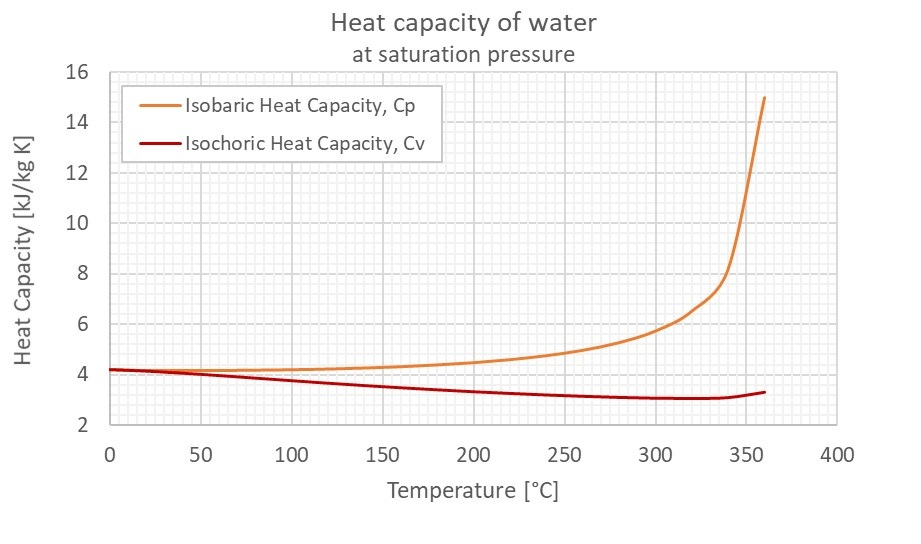
\includegraphics[scale=1.0]{Heat_capacity_C.jpg}
    \caption{\it{The heat capacity of water varying differently when kept at constant pressure compared to being kept at constant volume\cite{heat_cap}.}}
    \label{fig:heat_cap_water}
\end{figure}

This variation can be seen in Figure \ref{fig:heat_cap_water} where the heat capacity of water varies differently depending on which state variable is kept constant (either pressure of volume). \footnote{At temperatures close to $0^oC$ the difference in heat capacities Cp and Cv are approximately equal and only noticeably start to diverge from one another at temperatures close to $50^oC$.}\\

Now knowing the energy required to change the temperature of the substance, being able to measure the amount of energy being transferred to the substance is important (i.e. the efficiency). The efficiency of something is defined as the ratio of the useful work produced to the total energy expended. In the case of a refrigerator this is the ratio of the energy supplied to the cooling unit compared to the energy actually used to cool.\\

\begin{figure}[h!]
    \centering
    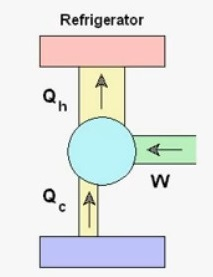
\includegraphics[scale=.75]{ref.jpg}
    \caption{\it{Energy movement through a refrigerator, transferring heat from a cold source, Qc, to a hot source, Qh, by providing work energy, W \cite{fridge}.}}
    \label{fig:fridge}
\end{figure}

Refrigerators operate by supplying work to move heat from a cold source to a hot source. The flow of heat for this process can be seen in Figure \ref{fig:fridge}. The efficiency ($\eta$) of the refrigeration process is given by;
\begin{equation}
    \eta = \frac{Q_C}{Q_H-Q_C}=\frac{Q_C}{Q_H/Q_C - 1}
\end{equation}

In the ideal circumstance where all of the work available is used to move heat is given by the Carnot efficiency\cite{carnot}. In this idealised case the efficiency is purely determined by the temperature ($T$) of the heat reservoirs.
\begin{equation}
        \eta_c = \frac{T_C}{T_H-T_C}=\frac{T_C}{T_H/T_C - 1}
\end{equation}
This is an idealised case describing the maximum efficiency, in reality it is impossible to reach this efficiency. 


% RPI Not a micro processor or micro controller but system on chip


\section*{Aims}
\begin{itemize}
    \item Build a circuit that measures the temperature of a substance and can control the on/off state of a Peltier heat pump\cite{peltier}. 
    \item Measure the cooling efficiency of the cooling circuit when cooling a known volume of water.
    \item Construct several convergence methods which determine the on/off state of the peltier depending on given inputs and compare their abilities at precisely controlling the temperature of the water.
\end{itemize}
\section*{Method}
% using the heat capacity of water at room tmp
\section*{Results and Discussion}

\subsection*{Discussion}

\section*{Areas of Further Research}


\section*{Conclusion}

\bibliographystyle{unsrt}
\bibliography{references}



\newpage
\appendix


\newpage
\section{Python Data Analysis Code}\label{ap:code}

\lstdefinestyle{mystyle}{
    backgroundcolor=\color{backcolour},   
    commentstyle=\color{codegreen},
    keywordstyle=\color{magenta},
    numberstyle=\tiny\color{codegray},
    stringstyle=\color{codepurple},
    basicstyle=\footnotesize,
    breakatwhitespace=false,         
    breaklines=true,                 
    captionpos=b,                    
    keepspaces=true,                 
    numbers=left,                    
    numbersep=5pt,                  
    showspaces=false,                
    showstringspaces=false,
    showtabs=false,                  
    tabsize=2
}
 
\lstset{style=mystyle}
 
% \begin{document}
% \lstinputlisting[language=python]{}
% \end{document}

\end{document}